\newpage
\lecture{3}{Продолжение борелевской истории и теорема Дынкина.}

\subsection{Структура минимальной сигма-алгебры.}

\begin{exercise}
    Пусть $\F$~--- семейство всех конечных подмножеств множества $X$. Найти $\sigma(\F)$.
\end{exercise}

\begin{solution}
    По определению $\sigma$"=алгебры $\forall A_1,\,A_2,\,\ldots\in\sigma(\F):\ \bigcup\limits_
        {n=1}^{\infty}A_n\in\sigma(\F)$. В частности, это верно для $\forall A_1, \, A_2,\,\ldots\in\F\Rightarrow$ в $\sigma(\F)$
    войдут все не более чем счётные подмножества множества $X$. Кроме того, $\forall A\in\sigma(\F)$ выполнено, что $A^C=X\setminus A\in\sigma(\F)
        \Rightarrow$ в $\sigma(\F)$ войдут также дополнения всех не более чем счётных множеств.

    Итак, $\CG=\{A\subset X:\ A \text{ или } A^C\text{ не более чем счётно}\}\subset\sigma(\F)$.
    Проверим что $\CG$~--- $\sigma$"=алгебра.
    \begin{enumerate}[label=\arabic*\degree.]
        \item $\varnothing\in\CG$~--- очевидно.
        \item $\forall A\in\CG:\ A^C\in\CG$ по построению.
        \item Если доказать, что $\forall A,\, B\in\CG:\ A\cap B\in\CG$, то сразу следует, что и
              $A\cup B = (A\cup B)^{CC}=(A^C\cap B^C)^C\in\CG$ (и наоборот, можно доказать лишь замкнутость по объединению и
              из неё сразу следует замкнутость по пересечению).

              Докажем сразу, что $\forall A_1,\,\ldots,\, A_n,\, \ldots\in\CG$ выполнено $\bigcup\limits_{n=1}^{\infty}A_n\in\CG$,
              то есть докажем разом замкнутость и то, что это именно $\sigma$"=алгебра.
              \begin{enumerate}[label=(a)]
                  \item Пусть $\forall n\in\N\ A_n$ не более чем счётно, тогда $\bigcup\limits_{n=1}^{\infty}A_n\in\CG$ так как
                        объединение так же не более чем счётно.
                  \item Если (a) не выполнено, то $\exists n\in\N:\ A_n$~--- более чем счётно, но так как $A_n\in\CG$, то
                        $A_n^C$~--- не более чем счётно, тогда
                        \[
                            \bigcup_{k=1}^{\infty}A_k=\left(\bigcup_{k=1}^{\infty}A_k\right)^{CC}=
                            \left(\bigcap_{k=1}^{\infty}A_k^C\right)^C.
                        \]
                        Теперь заметим, что в силу свойств пересечения $\bigcap\limits_{k=1}^{\infty}A_k^C\subset A_n^C$, то есть
                        $\bigcap\limits_{k=1}^{\infty}A_k^C$ тоже не более чем счётно, а значит $\bigcup\limits_{k=1}^{\infty}A_k\in\CG$,
                        так как его дополнение не более чем счётно.
              \end{enumerate}
    \end{enumerate}

    Тогда из $\F\subset \CG$ следует, что $\sigma(\F)\subset\CG$
    в силу минимальности по вложению $\sigma(\F)$. Откуда следует, что $\sigma(\F)=\CG$.

\end{solution}

\subsection{Структура борелевской сигма-алгебры.}

Напомним кратко понятия. $K_d$~--- семейство всех клеток в $\R^d$.
Борелевская сигма-алгебра $\FB(\R^d)=\sigma(\tau)$, где $\tau$~--- семейство всех открытых
множеств $U\subset  \R^d$, то есть, так называемая <<евклидова топология>>.

\begin{definition}
    Множество называется \mdef{борелевским} тогда и только тогда, когда оно является элементом
    борелевской сигма-алгебры.
\end{definition}

\begin{claim}
    $\sigma(K_d)=\FB(\R^d)$

    \begin{proof}

        Заметим, что $K_d\subset \FB(\R^d)$, в самом деле
        \[
            K = I_1\times\ldots\times I_d=
            =(I_1\times\R\times\ldots\times\R)\cap
            (\R\times I_2\times\ldots\times \R)\cap\ldots\cap
            (\R\times\R\times\ldots\times I_d),
        \]
        то есть представляем клетку как пересечение <<полос>> (см. рисунок \ref{fig:tapes}).

        \begin{figure}[!ht]
            \centering
            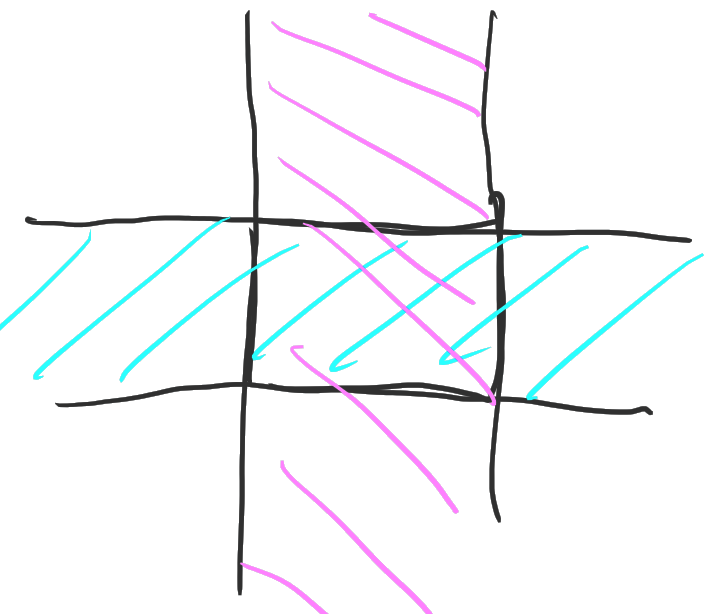
\includegraphics[width=0.25\textwidth]{tapes.png}
            \caption{Двумерные полоски.}
            \label{fig:tapes}
        \end{figure}

        Теперь посмотрим на промежутки:

        \begin{align*}
            I_1=\left[
            \begin{array}{ll}
                (a,\, b) \text{~--- открытое} \Rightarrow\in\FB(\R),\\
                \left[ a,\, b\right)=\bigcap\limits_{n=1}^{\infty} 
                \left(a-\dfrac{1}{n},\, b\right)\Rightarrow \in\FB(\R),\\ 
                \left( a,\, b\right]\text{~--- аналогично}\in\FB(\R),\\
                \left[a,\, b\right]\text{~--- дополнение к открытому}\Rightarrow\in\FB(\R).
            \end{array}
            \right .
        \end{align*}

        Аналогично множества $(I_1\times\R\times\ldots\times\R),\,
        (\R\times I_2\times\ldots\times \R),\,\ldots,\,
        (\R\times\R\times\ldots\times I_d)\in\FB(\R^d)$. А следовательно и их пересечение является
        борелевским множеством. 

        Итак, доказано, что $K_d\subset \FB(\R^d)\Rightarrow \sigma(K_d)\subset\FB(\R^d)$.

        Докажем теперь, что $\FB(\R^d)\subset \sigma(K_d)$. Так как 
        $\FB(\R^d)=\sigma(\tau)$ (см. определение), то достаточно доказать, что 
        $\tau\subset \sigma(K_d)$, в самом деле, если $\tau\subset \sigma(K_d)$, то 
        $\sigma(\tau)\subset \sigma(K_d)$ в силу минимальности $\sigma(\tau)$ по вложению.

        Пусть $U\in\tau$. Докажем, что $U\in\sigma(K_d)$.

        \begin{figure}[!ht]
            \centering
            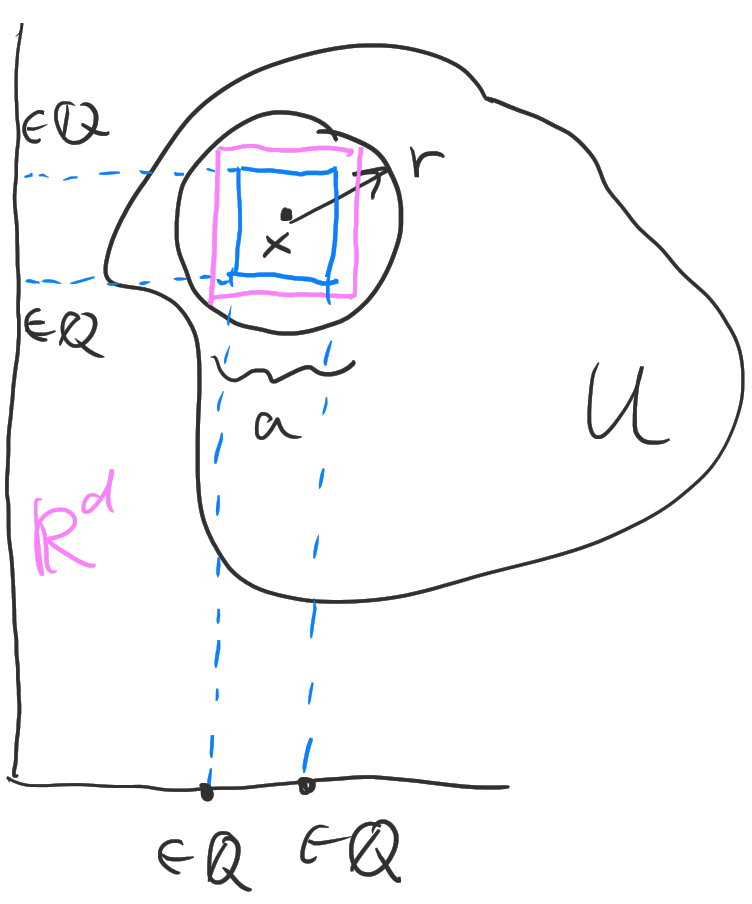
\includegraphics[width=0.6\textwidth]{upic.png}
            \caption{Множество $U$.}
            \label{fig:upic}
        \end{figure}

        $U$ открытое, поэтому $\forall x\in U\ \exists r>0:\ B_r(x)\subset U$, где $B_r(x)$~--- 
        $d$"=мерный шар радиуса $r$ с центром в точке $x$. Поймем какого размера должен быть 
        $d$"=мерный куб, чтобы его можно было вписать в данный шар. Должно выполнится следующее 
        неравенство: $\left(\dfrac{a}{2}\right)^2\cdot d\leqslant r^2$, где $a$~--- искомая сторона
        куба (неравенство следует из теоремы Пифагора: полудиагональ куба складывается из $d$ частей, 
        каждая длиной $\frac{a}{2}$). Откуда $a\leqslant \dfrac{2r}{\sqrt{d}}$. Таким образов любое 
        открытое множество можно представить в виде объединения таких кубиков (на рисунке \ref{fig:upic} это розовый квадрат),
        а кубики уже принадлежат семейству клеточных множеств.
        
        Но возникает проблема: такое объеденение кубиков может оказаться более чем счётным, поэтому сделаем финт ушами:
        сожмём кубик так, чтобы координаты его граней были рациональными (на рисунке это синий квадратик) и обзовем его $Q_x$.
        Множество таких кубов счётно, так как все такие кубы можно параметризовать точками $\Q^{2d}\Rightarrow$ данное семейство 
        счётно. 

        Тогда $\forall x\in U$ поставим в соответствие соответствующий куб $Q_x\subset B_r(x)\subset U$ и 
        $U=\bigcup\limits_{x\in U}\{x\}\subset \bigcup\limits_{x\in U}Q_x$~--- представимо в виде 
        не более чем счётного объединения, так как число кубов счётно и значит $U=\bigcup\limits_{x\in U}Q_x\in\sigma(K_d)$.

    \end{proof} 
\end{claim}

\subsection{Теорема Дынкина.}

\begin{definition}
    Семейство $\F\subset \CP(X)$ называется:
    \begin{enumerate}[label=\arabic*)]
        \item \mdef{$\pi$"=системой}, если $\forall A,\, B\in\F$ выполнено, что $A\cap B\in\F$;
        \item \mdef{$\lambda$"=системой}, если, во-первых, $\varnothing\in\F$, во-вторых,
        $\forall A\in\F$ выполнено, что $A^C\in\F$, а также для любых попарно непересекающихся 
        $D_1,\, \ldots,\, D_n,\,\ldots\in\F$ выполнено $\bigsqcup\limits_{k=1}^{\infty} D_k\in\F$.
    \end{enumerate}
\end{definition}

\begin{exercise}
    $\lambda$"=система в общем случае не всегда является $\pi$"=системой. Например, пусть 
    $X=\{1,\,2,\,3,\,4\}$ и 
    \[
        \F = \{\varnothing,\, X,\, \{1,\,2\},\, \{1,\,3\},\,\{1,\,4\},\,\{2,\,3\},\,\{2,\,4\},\,\{3,\,4\}\}.    
    \]
    Легко видеть, что это $\lambda$"=система, но не $\pi$"=система, так как $\F$ не замкнута относительно пересечения.
\end{exercise}

\begin{exercise}
    Другой пример. Пусть $X=\R^2,\ \F = \{\R\times A:\ A\subset \R\}\cup \{A\times \R:\ A\subset \R\}$~---
    семейство горизонтальных и вертикальных полос.
    \begin{enumerate}
        \item $\F$~--- не $\pi$"=система, так как $(\R\times A)\cap (B\times \R)=B\times A\notin \F,\ A,\, B\neq \R$.
        \item Легко видеть, что $\F$~--- $\lambda$"=система.
    \end{enumerate}
\end{exercise}

На прошлой лекции было доказано следующее утверждение (теперь в новой терминологии):
\begin{claim}
    $\F\subset\CP(X)$ является $\sigma$"=алгеброй тогда и только тогда, когда $\F$ 
    одновременно является $\pi$"=системой и $\lambda$"=системой.
\end{claim}

\begin{figure}[!ht]
    \centering
    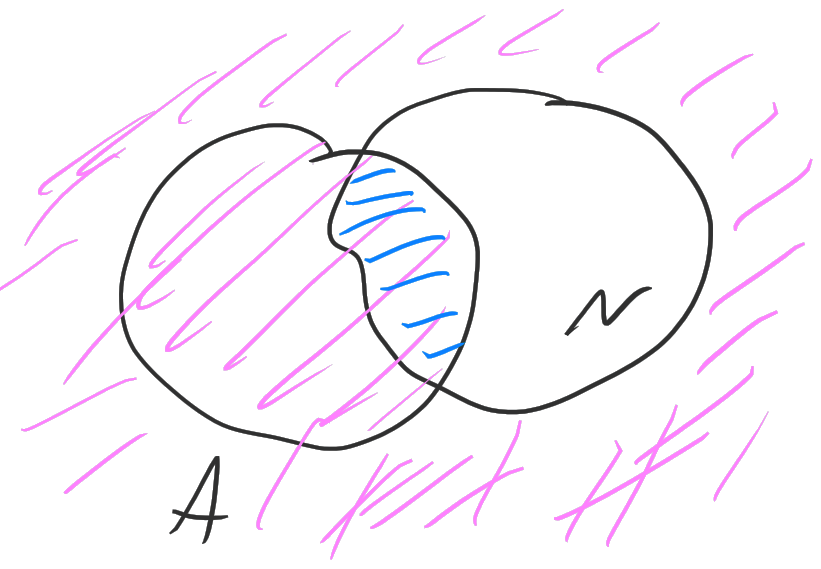
\includegraphics[width=0.5\textwidth]{sets.png}
    \caption{К теореме Дынкина (\ref{theorem:dynkin})}
    \label{fig:sets}
\end{figure}

\begin{theorem}[Дынкин]
    \label{theorem:dynkin}

    Пусть $\F\subset\CP(X)$~--- $\pi$"=система, $\CE\subset\CP(X)$~--- $\lambda$"=система и
    $\F\subset\CE$. Тогда $\sigma(\F)\subset\CE$ (равенство возможно).

    \begin{proof}
        Пусть $\CD\subset \CP(X)$~--- пересечение всех $\lambda$"=систем $\CG\subset\CP(X)$, 
        таких что $\F\subset\CG$. Докажем, что $\sigma(\F)\subset\CD$, для этого достаточно доказать, 
        что $\CD$ является $\sigma$"=алгеброй (снова в силу минимальности).

        Заметим, что $\CD$~--- $\lambda$"=система (доказывается так же как и факт о том, что пересечение сигма-алгебр является
        сигма-алгеброй). Тогда достаточно показать, что $\CD$~--- $\pi$"=система, то есть, что 
        $\forall M,\, N\in\CD$ выполняется, что $M\cap N\in\CD$.

        Введем обозначение: $\CH(M)=\{N\in\CD:\: M\cap N\in\CD\}$, где $M$~--- любой элемент $\CD$. То есть 
        условие о замкнутости по пересечению можно переформулировать так: $\forall M\in\CD$ выполнено $\CH(M)=\CD$.

        \begin{lemma}
            $\forall N\in\CD$ верно, что $\CH(N)$ является $\lambda$"=системой.

            \begin{proof}
                Во-первых, $\varnothing\in\CH(N)$, так как $\forall M\in\CD:\ \varnothing\cap M=\varnothing\in\CD$ по определению.

                Во-вторых, докажем, что $\CH(N)$ замкнуто относительно взятия дополнений. Пусть $A\in\CH(N)$. 
                Заметим, что
                \begin{equation}
                    \label{eq:lemmastate}
                    A\in\CH(N)\ \Leftrightarrow\ A\cap N\in\CD.
                \end{equation}
                И в частности 
                \[
                    A^C\in\CH(N)\ \Leftrightarrow\ A^C\cap N\in\CD.    
                \]
                Правое условие, в силу того, что $\CD$~--- $\lambda$"=система эквивалентно тому, что 
                $(A^C\cap N)^C\in\CD$ (из замкнутости по дополнению). Но $(A^C\cap N)^C=A\cup N^C=(A\cap N)\sqcup N^C\in\CD$ 
                (см. рис. \ref{fig:sets}). Итак, $A^C\in\CH(N)$.

                Докажем замкнутость относительно дизъюнктных объединений. Пусть 
                $A_1,\,\ldots,\,A_n,\,\ldots\in\CH(N)$ попарно не пересекаются. Тогда:
                \[
                    \left(\bigsqcup_{n=1}^{\infty}A_n\right)\cap N=\bigsqcup_{n=1}^{\infty}\left(A_n\cap N\right)\in \CD,
                \]
                так как $A_n\cap N\in\CD$ (см. условие \eqref{eq:lemmastate}) и $\CD$~--- $\lambda$"=система.

            \end{proof}
        \end{lemma}

        Пусть $M\in\F\subset\CD$ (по построению). Зададимся вопросом: для каких $N\in\CD$ выполнено, что $M\cap N\in\CD$?
        Если $N\in\F$, то $M\cap N\in\F$, так как $\F$~--- $\pi$"=система. Поэтому $\forall N\in\F$
        выполнено $N\in\CH(M)$, то есть $\F\subset\CH(M)$, а значит $\CH(M)$~--- одна из $\lambda$"=систем, включающих в себя 
        $\F$, следовательно, в силу минимальности по вложению, $\CD\subset\CH(M)$ для $\forall M\in\F$, 
        то есть $\forall N\in\CD,\, \forall M\in\F$ выполнено $M\cap N\in\CD$. А значит $\forall N\in\CD$ выполнено $\F\subset\CH(N)$, и 
        снова в силу минимальности $\CD\subset \CH(N)$. Итак, $\forall N,\, M\in\CD$ выполнено $M\cap N\in\CD$.
        
    \end{proof}
\end{theorem}

